\section{Specifying synchronisations}
\label{sec:spec}

In this section we describe how synchronisations can be formally specified.
For ease of exposition, we start by considering \emph{heterogeneous binary}
synchronisation in this section, i.e.~where every synchronisation is between
\emph{two} invocations of \emph{different} operations.  We generalise at the
end of this section.

We assume that the synchronisation object has two operations, each of which
has a single parameter, with signatures as follows.
%
\begin{scala}
def op£\s1£(x£\s1£: A£\s1£): B£\s1£
def op£\s2£(x£\s2£: A£\s2£): B£\s2£
\end{scala}
%
(We can model a concrete operation that takes $k \ne 1$ parameters by an
operation that takes a $k$-tuple as its parameter.  We identify a 0-tuple with
the unit value, but will sometimes omit that value in examples.)
%
In addition, the synchronisation object might have some state, |state: S|.
Each invocation of~|op|\s1 must synchronise with an invocation of~|op|\s2, and
vice versa.  The result of each invocation may depend on the two parameters
|x|$_1$ and |x|$_2$ and the current state.  In addition, the state may be
updated.  The external behaviour is consistent with the synchronisation
happening atomically at some point within the duration of both operation
invocations (which implies that the invocations must overlap): we refer to this
point as the \emph{synchronisation point}.

Each synchronisation object can be specified using a \emph{synchronisation
  specification object} with the following signature.
%
\begin{scala}
class Spec{
  def sync(x£\s1£: A£\s1£, x£\s2£: A£\s2£): (B£\s1£, B£\s2£)
}
\end{scala}
%
The idea is that if two invocations |op|\s1|(x|\s1|)| and |op|\s2|(x|\s2|)|
synchronise, then the results |y|\s1 and |y|\s2 of the invocations are such
that $\sm{sync}(\sm x_1, \sm x_2)$ could return the pair |(y|\s1|, y|\s2|)|.
(We allow |sync| to be nondeterministic; but in all our examples it will be
deterministic.)  The specification object might have some private state that
is accessed and updated within~|sync|.  Note that invocations of |sync| occur
\emph{sequentially}.

We formalise below what it means for a synchronisation object to satisfy the
requirements of a synchronisation specification object.  But first, we give
some examples to illustrate the style of specification. 

A generic definition of a specification object might take the following form: 
%
\begin{scala}
class Spec{
  private var state: S
  def sync(x£\s1£: A£\s1£, x£\s2£: A£\s2£): (B£\s1£, B£\s2£) = {
    require(guard(x£\s1£, x£\s2£, state))
    val res£\s1£ = f£\s1£(x£\s1£, x£\s2£, state); val res£\s2£ = f£\s2£(x£\s1£, x£\s2£, state)
    state = update(x£\s1£, x£\s2£, state)
    (res£\s1£, res£\s2£)
  }
}
\end{scala}
%
The object has some local state, which persists between invocations.  The
|require| clause of |sync| specifies a precondition for the synchronisation to
take place.  The values |res|\s1 and |res|\s2 represent the results that
should be returned by the corresponding invocations of~|op|\s1 and~|op|\s2,
respectively.  The function |update| describes how the local state should be
updated. 

For example, consider a synchronous channel with operations
\begin{scala}
def send(x: A): Unit
def receive(u: Unit): A
\end{scala}
%
(Note that we model the |receive| operation as taking a parameter of type
|Unit|, in order to fit our uniform setting.) 
%
This can be specified using a synchronisation specification object
with empty state:
%
\begin{scala}
class SyncChanSpec[A]{
  def sync(x: A, u: Unit): (Unit, A) = ((), x)
}
\end{scala}
%
If |send(x)| synchronises with |receive(())|, then the former receives the
unit value~|()|, and the latter receives~|x|. 

As another example, consider a filtering channel.
\begin{scala}
class FilterChan[A]{
  def send(x: A): Unit
  def receive(p: A => Boolean): A
}
\end{scala}
%
Here the |receive| operation is passed a predicate~|p| describing a required
property of any value received.  This can be specified using a specification
object with operation
%
\begin{scala}
def sync(x: A, p: A => Boolean): (Unit, A) = { require(p(x)); ((), x) }
\end{scala}
%
The |require| clause specifies that invocations |send(x)| and |receive(p)| can
synchronise only if |p(x)|.

As an example illustrating the use of state in the synchronisation object,
recall the synchronous channel with a sequence counter, |SyncChanCounter|,
from the introduction.  This can be specified using the following
specification object.
%
\begin{scala}
class SyncChanCounterSpec[A]{
  private var counter = 0
  def sync(x: A, u: Unit): (Int, (A, Int)) = {
    counter += 1; (counter, (x, counter))
  }
}
\end{scala}

%%%%%%%%%%

\subsection{Linearisability}
\label{sec:specification-linearisability}

We formalise below precisely the allowable behaviours captured by a particular
synchronisation specification object.  Our definition has much in common with
the well known notion of \emph{linearisation}~\cite{herlihy-wing}, used for
specifying concurrent datatypes; so we start by reviewing that notion.  There
are a number of equivalent ways of defining linearisation: we choose a way
that will be convenient subsequently.

A \emph{concurrent history} of an object~$o$ (either a concurrent datatype or
a synchronisation object) records the calls and returns of operation
invocations on~$o$.  It is a sequence of events of the following forms:
%
\begin{itemize}
\item $\call.op^i(x)$, representing a call of operation~$op$ with
  parameter~$x$;
\item $\return.op^i \:: y$, representing a return of an invocation of~$op$,
  giving result~$y$.
\end{itemize}
%
Here $i$ is a \emph{invocation identity}, used to identify a particular
invocation, and to link the $\call$ and corresponding~$\return$.  In order to
be well formed, each invocation identity must appear on at most one $\call$
event and at most one $\return$ event; and for each event $\return.op^i\::y$,
the history must contain an earlier event $\call.op^i(x)$, i.e.~for the same
operation and invocation identity.  We consider only well formed histories
from now on.  

We say that a $\call$ event and a $\return$ event \emph{match}
if they have the same invocation identifier.  A concurrent history is
\emph{complete} if for every $\call$ event, there is a matching $\return$
event, i.e.~no invocation is still pending at the end of the history.

For example, consider the following complete concurrent history of a
concurrent object that is intended to implement a queue, with operations |enq|
and~|deq|.
%
\begin{eqnarray*}
h & = & 
  \seq{\begin{align}
    \call.\sm{enq}^1(5),\; \call.\sm{enq}^2(4),\; \call.\sm{deq}^3(), \\
    \return.\sm{enq}^1\::(),\; \return.\sm{deq}^3\::4,\;
    \return.\sm{enq}^2\::() }.
    \end{align}
\end{eqnarray*}
%
This history is illustrated by the timeline in Figure~\ref{fig:lin-timeline}:
here, time runs from left to right; each horizontal line represents an
operation invocation, with the left-hand end representing the $\call$ event,
and the right-hand end representing the $\return$ event. 

%%%%%

\begin{figure}
\unScalaMid
\def\X{node{$\cross$}}
\begin{center}
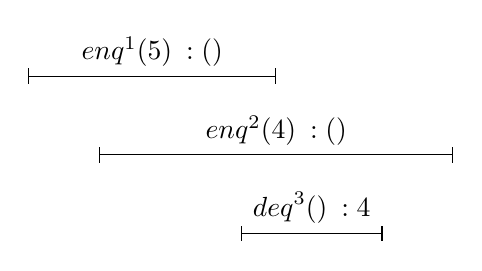
\begin{tikzpicture}[xscale = 0.9]
\draw[|-|] (0,0) -- node[above] {$\sm{enq}^1(5)\::()$} (3.5,0);
\draw (2.5,0) \X;
\draw[|-|] (1,-1) -- node[above] {$\sm{enq}^2(4)\::()$} (6,-1);
\draw (2,-1) \X;
\draw[|-|] (3,-2) -- node[above] {$\sm{deq}^3()\::4$} (5,-2);
\draw (4,-2) \X;
\end{tikzpicture}
\end{center}
\caption{Timeline representing the linearisation example.}
\label{fig:lin-timeline}
\scalaMid
\end{figure}

%%%%%

Linearisability is specified with respect to a specification object~$Spec$,
with the same operations (and signatures) as the concurrent object in
question.  A history of the specification object is a sequence of events of
the form:
%
\begin{itemize}
\item $op^i(x)\::y$ representing an invocation of operation~$op$ with
  parameter~$x$, returning result~$y$; again $i$~is an invocation identity,
  which must appear at most once in the history.
\end{itemize}
%
A history is \emph{legal} if it is consistent with the definition of~$Spec$,
i.e.~for each invocation, the precondition is satisfied, and the return value
is as for the definition of the operation in~$Spec$.

For example, consider the history
\begin{eqnarray*}
h_s & = & \seq{\sm{enq}^2(4)\::(),\; \sm{enq}^1(5)\::(),\; \sm{deq}^3()\::4}.
\end{eqnarray*}
%
This is a legal history for a specification object that represents a queue.
This history is illustrated by the ``$\cross$''s in
Figure~\ref{fig:lin-timeline}.

Let $h$ be a complete concurrent history, and let $h_s$ be a legal history of
the specification object.  We say that $h$ and~$h_s$ \emph{correspond} if they
contain the same invocations, i.e., for each $\call.op^i(x)$ and
$\return.op^i\::y$ in $h$,\, $h_s$ contains $op^i(x)\::y$, and vice versa.  We
say that $h$ and~$h_s$ are \emph{compatible} if there is some way of
interleaving the two histories (i.e.~creating a history containing the events
of~$h$ and~$h_s$, preserving the order of events) such that each $op^i(x)\::y$
occurs between $\call.op^i(x)$ and $\return.op^i\::y$.  Informally, this
indicates that the invocations of~$h$ appeared to take place in the order
described by~$h_s$, and that this order is consistent with the specification
object.

Continuing the running example, the histories $h$ and~$h_s$ are compatible, as
evidenced by the interleaving
\[
\seq{\begin{align}
  \call.\sm{enq}^1(5),\; \call.\sm{enq}^2(4),\; 
  \sm{enq}^2(4)\::(),\; \sm{enq}^1(5)\::(),\;   \call.\sm{deq}^3(), \\
  \return.\sm{enq}^1\::(),\; \sm{deq}^3\::4,\; 
  \return.\sm{deq}^3\::4,\; \return.\sm{enq}^2\::() },
  \end{align}
\]
as illustrated in  Figure~\ref{fig:lin-timeline}.

We say that a complete history~$h$ is \emph{linearisable} with respect to
$Spec$ if there is a corresponding legal history~$h_s$ of~$Spec$ such that $h$
and~$h_s$ are compatible.  

A concurrent history might not be complete, i.e.~it might have some pending
invocations that have been called but have not returned.  An \emph{extension}
of a history~$h$ is formed by adding zero or more $\return$ events
corresponding to pending invocations.  We write $complete(h)$ for the
subsequence of~$h$ formed by removing all $\call$ events corresponding to
pending invocations.
%
We say that a (not necessarily complete) concurrent history~$h$ is
\emph{linearisable} if there is an extension~$h'$ of~$h$ such that
$complete(h')$ is linearisable.  We say that a concurrent object is
linearisable if all of its histories are linearisable. 

%%%%%

\subsection{Synchronisation linearisability}

We now adapt the definition of linearisability to synchronisations.  We
consider a concurrent history of the synchronisation object~$Sync$.  The
history contains $\call$ and $\return$ events, as in the previous subsection;
in the case of binary synchronisation, the events correspond to the
operations~$\op_1$ and~$\op_2$.

For example, the following is a complete history of the synchronous channel
from earlier, and is illustrated in Figure~\ref{fig:sync-timeline}:
\begin{eqnarray*}
h & = & 
\seq{\begin{align}
  \call.\sm{send}^1(8),\; \call.\sm{send}^2(8),\; \call.\sm{receive}^3(()),\;
  \return.\sm{receive}^3\::8,\; \\
  \call.\sm{receive}^4(()),\; \return.\sm{send}^1\::(),\;
  \call.\sm{send}^5(9),\; \return.\sm{receive}^4\::9,\; \\
  \call.\sm{receive}^6(()),\; \return.\sm{send}^2\::(), \;
  \return.\sm{send}^5\::(),\; \return.\sm{receive}^6\::8 } .
  \end{align}
\end{eqnarray*}

%%%%%

\begin{figure}
\unScalaMid
\begin{center}
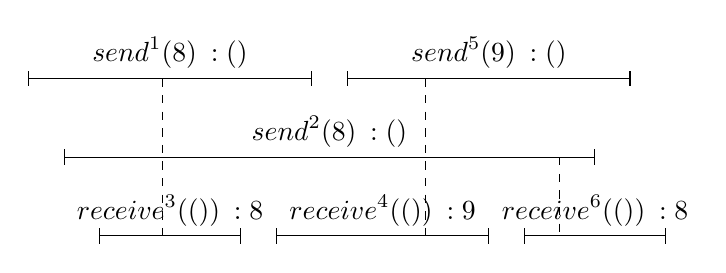
\begin{tikzpicture}[xscale = 0.9]
\draw[|-|] (0,0) -- node[above] {$\sm{send}^1(8)\::()$} (4,0);
\draw[|-|] (4.5,0) -- node[above] {$\sm{send}^5(9)\::()$} (8.5,0);
\draw[|-|] (0.5,-1) -- node[above] {$\sm{send}^2(8)\::()$} (8,-1);
\draw[|-|] (1,-2) -- node[above] {$\sm{receive}^3(())\::8$} (3,-2);
\draw[|-|] (3.5,-2) -- node[above] {$\sm{receive}^4(())\::9$} (6.5,-2);
\draw[|-|] (7,-2) -- node[above] {$\sm{receive}^6(())\::8$} (9,-2);
\draw (1.9,0) \X; \draw (1.9,-2) \X; 
\draw[dashed] (1.9,0) -- (1.9,-2); % sync 1 and 3
\draw (5.6,0) \X; \draw (5.6,-2) \X; 
\draw[dashed] (5.6,0) -- (5.6,-2); % sync 4 and 5
\draw (7.5,-1) \X; \draw (7.5,-2) \X; 
\draw[dashed] (7.5,-1) -- (7.5,-2); % sync 2 and 6 
\end{tikzpicture}
\end{center}
\caption{Timeline representing the synchronisation example.}
\label{fig:sync-timeline}
\scalaMid
\end{figure}


A history of a synchronisation specification object $Spec$ is a sequence of
events of the form $\sync^{i_1, i_2}(x_1, x_2)\:: (y_1, y_2)$, representing an
invocation of |sync| with parameters $(x_1, x_2)$ and result $(y_1,y_2)$.  The
event's invocation identity is~$(i_1,i_2)$: each of~$i_1$ and~$i_2$ must
appear at most once in the history.  Informally, an event $\sync^{i_1,
  i_2}(x_1, x_2)\:: (y_1, y_2)$ corresponds to a synchronisation between
invocations $\op_1^{i_1}(x_1)\::y_1$ and $\op_2^{i_2}(x_2)\::y_2$ in a history
of the corresponding synchronisation object.

A history is \emph{legal} if is consistent with the specification object.  
%
For example, the following is a legal history of |SyncChanSpec|.
\begin{eqnarray*}
h_s & = & 
\seq{
 \sm{sync}^{1,3}(8,()) \:: ((), 8), \;
 \sm{sync}^{5,4}(9,()) \:: ((), 9), \;
 \sm{sync}^{2,6}(8,()) \:: ((), 8) } .
\end{eqnarray*}
The history is illustrated by the ``$\cross$''s in
Figure~\ref{fig:sync-timeline}: each event corresponds to the synchronisation
of two operations, so is depicted by two ``$\cross$''s on the corresponding
operations, linked by a dashed vertical line.  This particular synchronisation
specification object is stateless, so in fact any permutation of this history
would also be legal (but not all such permutations will be compatible with the
history of the synchronisation object); but the same will not be true in
general of a specification object with state.

Let $h$ be a complete history of the synchronisation object~$Sync$.  We say
that a legal history~$h_s$ of~$Spec$ \emph{corresponds} to~$h$ if:
%
\begin{itemize}
\item For each |sync| event with identity~$(i_1,i_2)$ in~$h_s$,\, $h$ contains
  an invocation of~$\op_1$ with identity~$i_1$ and an invocation of~$\op_2$ with
  identity~$i_2$;

\item For each invocation of~$\op_1$ with identity~$i_1$ in~$h$,\, $h_s$
  contains a |sync| event with identity~$(i_1,i_2)$ for some~$i_2$;

\item For each invocation of~$\op_2$ with identity~$i_2$ in~$h$,\, $h_s$
  contains a |sync| event with identity~$(i_1,i_2)$ for some~$i_1$.
\end{itemize}
%
%% Informally, a |sync| event with identity~$(i_1,i_2)$ represents that the
%% invocations $op_1^{i_1}$ and $op_2^{i_2}$ synchronise.

We say that a complete history $h$ of~$Sync$ and a corresponding legal history
$h_s$ of~$Spec$ are \emph{synchronisation-compatible} if there is some way of
interleaving them such that each event $\sync^{i_1, i_2}(x_1, x_2)\:: (y_1,
y_2)$ occurs between $\call.\op_1^{i_1}(x_1)$ and $\return.\op_1^{i_1}\::y_1$,
and between $\call.\op_2^{i_2}(x_2)$ and $\return.\op_2^{i_2}\::y_2$.
%
In~the running example, the histories~$h$ and~$h_s$ are synchronisation
compatible, as shown by the interleaving in Figure~\ref{fig:sync-timeline}.

We say that a complete history $h$ of~$Sync$ is
\emph{synchronisation-linearisable} if there is a corresponding legal history
$h_s$ of~$Spec$ such that $h$ and~$h_s$ are synchronisation compatible.

We say that a (not necessarily complete) concurrent history~$h$ is
\emph{synchronisation-linearisable} if there is an extension~$h'$ of~$h$ such
that $complete(h')$ is synchronisation-linearisable.  We say that a
synchronisation object is synchronisation-linearisable if all of its histories
are synchronisation-linearisable.

%% Following definition of linearisation.  History of synchronisation object,
%% containing call and return events, with matching invocation indices,
%% e.g. $call.\sm{op}_1^{i_1}(x_1)$ and $return.\sm{op}_1^{i_1}: y_1$; indiced
%% otherwise distinct.  History of sequential specification object, with events
%% representing (atomic) invocations of sync, labelled with a pair of invocation
%% indices, e.g.~$\sm{sync}^{i_1, i_2}(x_1, x_2): (y_1, y_2)$.  No invocation
%% index is repeated in the history.  Define ``legal'' in the normal way.  Define
%% interleaving of concurrent and sequential history: each |sync| has to be
%% between the corresponding $call$ and $return$ for each of the two invocations.

%% Maybe call this \emph{synchronisation linearisation}. 

\framebox{Is the definition compositional?}  I think so.
